\section{Introduction}
In 2000, Wood publishes a paper: The Feasibility of Magnetic Recording at 1 Terabits Per Square Inch~\cite{Wood2000}. It says, that conventional recording would reach a limit at around 1 Terabit/in$^2$.

However, in 2009, he admits~\cite{Wood2009} the current hard disk drive (HDD) technology is already reaching this limit. Wood is right that to assure continued capacity growth in HDD need alternative technologies: heat-assisted magnetic recording (HAMR)~\cite{Rottmeyer} and bit patterned media (BPM)~\cite{Terris}. 

Toward proof of the concept, the Advanced Storage Technology Consortium (ASTC)~\cite{ASTC} released the 2014 roadmap for HDD area density as shown in Fig.\,\ref{fig_astc}.

\begin{figure}[!hbt]
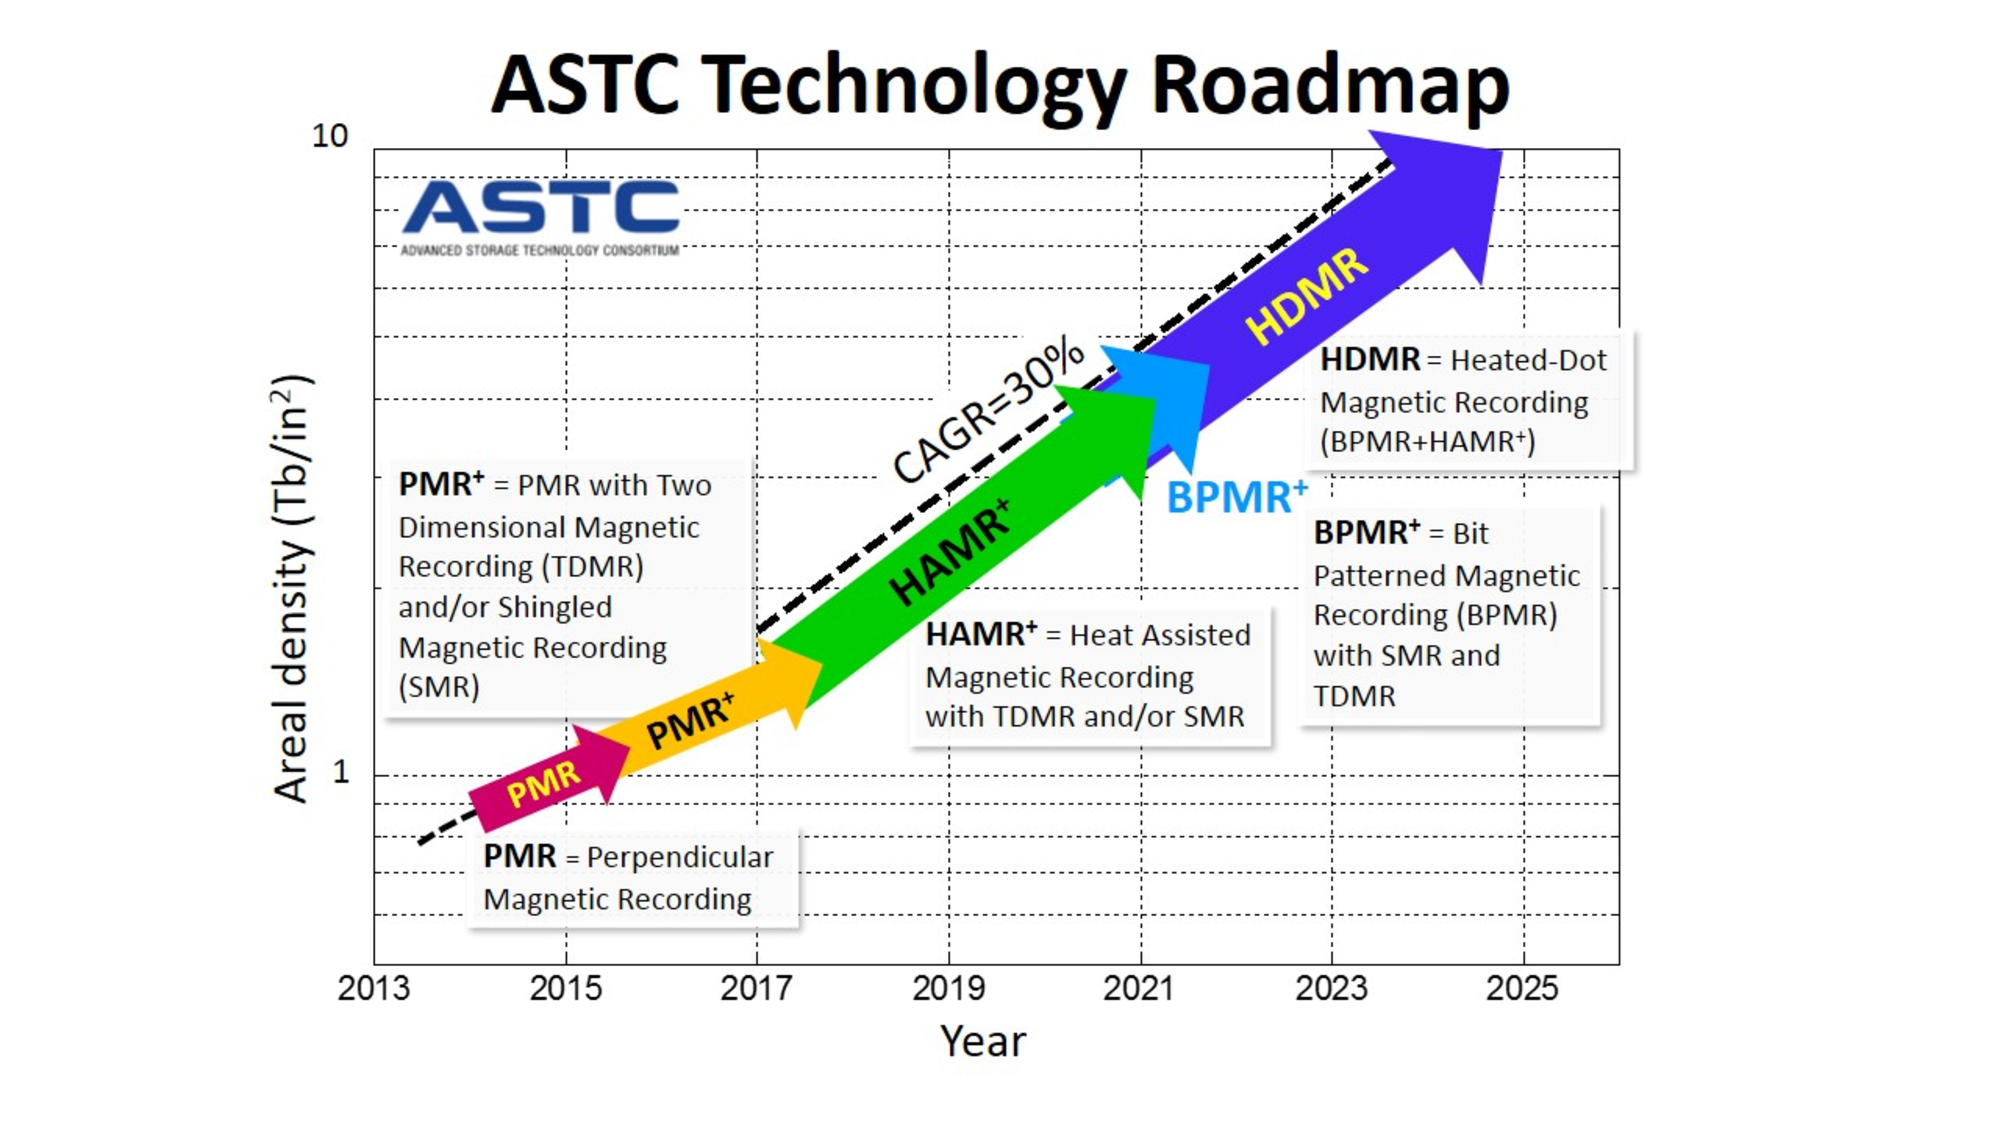
\includegraphics[height=0.25\textheight]{ASTC}
\caption{Data synchronization between two devices}
\label{fig_astc}
\end{figure}

Figure\,\ref{fig_astc} shows the current HDD technology is Perpendicular recording~\cite{HGST} and future HDD technologies currently in development include: HAMR and BPM with Two Dimensional Magnetic Recording (TDMR)~\cite{Krishnan} and Shingled Magnetic Recording (SMR)~\cite{Gibson}

\subsection{HAMR} 
HAMR uses temperature as well as magnetism. Currently to increase the recording density, it requires reduction magnetic bit size. Which will be difficult to magnetise. HARM solves this problem by heating magnetic bit just before the write head applies its magnetic field. With this heat, the magnetic material will reach the point when it is easy to change its magnetic property.
\subsection{BPM}


